%% Run LaTeX on this file several times to get Table of Contents,
%% cross-references, and citations.

\documentclass[11pt]{book}
\usepackage{gvv}
\usepackage{gvv-book-bkup}
%\usepackage{Wiley-AuthoringTemplate}
\usepackage[sectionbib,authoryear]{natbib}% for name-date citation comment the below line
%\usepackage[sectionbib,numbers]{natbib}% for numbered citation comment the above line

%%********************************************************************%%
%%       How many levels of section head would you like numbered?     %%
%% 0= no section numbers, 1= section, 2= subsection, 3= subsubsection %%
\setcounter{secnumdepth}{3}
%%********************************************************************%%
%%**********************************************************************%%
%%     How many levels of section head would you like to appear in the  %%
%%				Table of Contents?			%%
%% 0= chapter, 1= section, 2= subsection, 3= subsubsection titles.	%%
\setcounter{tocdepth}{2}
%%**********************************************************************%%
\setcounter{tocdepth}{3}
%\includeonly{ch01}
\makeindex

\begin{document}

\frontmatter
%%%%%%%%%%%%%%%%%%%%%%%%%%%%%%%%%%%%%%%%%%%%%%%%%%%%%%%%%%%%%%%%
%% Title Pages
%% Wiley will provide title and copyright page, but you can make
%% your own titlepages if you'd like anyway
%% Setting up title pages, type in the appropriate names here:

\booktitle{CBSE Math}

\subtitle{Made Simple}

\AuAff{G. V. V. Sharma}

%% \\ will start a new line.
%% You may add \affil{} for affiliation, ie,
%\authors{Robert M. Groves\\
%\affil{Universitat de les Illes Balears}
%Floyd J. Fowler, Jr.\\
%\affil{University of New Mexico}
%}

%% Print Half Title and Title Page:
%\halftitlepage
\titlepage

%%%%%%%%%%%%%%%%%%%%%%%%%%%%%%%%%%%%%%%%%%%%%%%%%%%%%%%%%%%%%%%%
%%Copyright Page

\begin{copyrightpage}{2023}
%Title, etc
\end{copyrightpage}

% Note, you must use \ to start indented lines, ie,
% 
% \begin{copyrightpage}{2004}
% Survey Methodology / Robert M. Groves . . . [et al.].
% \       p. cm.---(Wiley series in survey methodology)
% \    ``Wiley-Interscience."
% \    Includes bibliographical references and index.
% \    ISBN 0-471-48348-6 (pbk.)
% \    1. Surveys---Methodology.  2. Social 
% \  sciences---Research---Statistical methods.  I. Groves, Robert M.  II. %
% Series.\\

% HA31.2.S873 2004
% 001.4'33---dc22                                             2004044064
% \end{copyrightpage}

%%%%%%%%%%%%%%%%%%%%%%%%%%%%%%%%%%%%%%%%%%%%%%%%%%%%%%%%%%%%%%%%
%% Only Dedication (optional) 

%\dedication{To my parents}

\tableofcontents

%\listoffigures %optional
%\listoftables  %optional

%% or Contributor Page for edited books
%% before \tableofcontents

%%%%%%%%%%%%%%%%%%%%%%%%%%%%%%%%%%%%%%%%%%%%%%%%%%%%%%%%%%%%%%%%
%  Contributors Page for Edited Book
%%%%%%%%%%%%%%%%%%%%%%%%%%%%%%%%%%%%%%%%%%%%%%%%%%%%%%%%%%%%%%%%

% If your book has chapters written by different authors,
% you'll need a Contributors page.

% Use \begin{contributors}...\end{contributors} and
% then enter each author with the \name{} command, followed
% by the affiliation information.

% \begin{contributors}
% \name{Masayki Abe,} Fujitsu Laboratories Ltd., Fujitsu Limited, Atsugi, Japan
%
% \name{L. A. Akers,} Center for Solid State Electronics Research, Arizona State University, Tempe, Arizona
%
% \name{G. H. Bernstein,} Department of Electrical and Computer Engineering, University of Notre Dame, Notre Dame, South Bend, Indiana; formerly of
% Center for Solid State Electronics Research, Arizona
% State University, Tempe, Arizona 
% \end{contributors}

%%%%%%%%%%%%%%%%%%%%%%%%%%%%%%%%%%%%%%%%%%%%%%%%%%%%%%%%%%%%%%%%
% Optional Foreword:

%\begin{foreword}
%\lipsum[1-2]
%\end{foreword}

%%%%%%%%%%%%%%%%%%%%%%%%%%%%%%%%%%%%%%%%%%%%%%%%%%%%%%%%%%%%%%%%
% Optional Preface:

%\begin{preface}
%\lipsum[1-1]
%\prefaceauthor{}
%\where{place\\
% date}
%\end{preface}

% ie,
% \begin{preface}
% This is an example preface.
% \prefaceauthor{R. K. Watts}
% \where{Durham, North Carolina\\
% September, 2004}

%%%%%%%%%%%%%%%%%%%%%%%%%%%%%%%%%%%%%%%%%%%%%%%%%%%%%%%%%%%%%%%%
% Optional Acknowledgments:

%\acknowledgments
%\lipsum[1-2]
%\authorinitials{I. R. S.}  

%%%%%%%%%%%%%%%%%%%%%%%%%%%%%%%%
%% Glossary Type of Environment:

% \begin{glossary}
% \term{<term>}{<description>}
% \end{glossary}

%%%%%%%%%%%%%%%%%%%%%%%%%%%%%%%%
%\begin{acronyms}
%\acro{ASTA}{Arrivals See Time Averages}
%\acro{BHCA}{Busy Hour Call Attempts}
%\acro{BR}{Bandwidth Reservation}
%\acro{b.u.}{bandwidth unit(s)}
%\acro{CAC}{Call / Connection Admission Control}
%\acro{CBP}{Call Blocking Probability(-ies)}
%\acro{CCS}{Centum Call Seconds}
%\acro{CDTM}{Connection Dependent Threshold Model}
%\acro{CS}{Complete Sharing}
%\acro{DiffServ}{Differentiated Services}
%\acro{EMLM}{Erlang Multirate Loss Model}
%\acro{erl}{The Erlang unit of traffic-load}
%\acro{FIFO}{First in - First out}
%\acro{GB}{Global balance}
%\acro{GoS}{Grade of Service}
%\acro{ICT}{Information and Communication Technology}
%\acro{IntServ}{Integrated Services}
%\acro{IP}{Internet Protocol}
%\acro{ITU-T}{International Telecommunication Unit -- Standardization sector}
%\acro{LB}{Local balance}
%\acro{LHS}{Left hand side}
%\acro{LIFO}{Last in - First out}
%\acro{MMPP}{Markov Modulated Poisson Process}
%\acro{MPLS}{Multiple Protocol Labeling Switching}
%\acro{MRM}{Multi-Retry Model}
%\acro{MTM}{Multi-Threshold Model}
%\acro{PASTA}{Poisson Arrivals See Time Averages}
%\acro{PDF}{Probability Distribution Function}
%\acro{pdf}{probability density function}
%\acro{PFS}{Product Form Solution}
%\acro{QoS}{Quality of Service}
%\acro{r.v.}{random variable(s)}
%\acro{RED}{random early detection}
%\acro{RHS}{Right hand side}
%\acro{RLA}{Reduced Load Approximation}
%\acro{SIRO}{service in random order}
%\acro{SRM}{Single-Retry Model}
%\acro{STM}{Single-Threshold Model}
%\acro{TCP}{Transport Control Protocol}
%\acro{TH}{Threshold(s)}
%\acro{UDP}{User Datagram Protocol}
%\end{acronyms}

\setcounter{page}{1}

\begin{introduction}
This book links high school coordinate geometry to linear algebra and matrix analysis through solved problems.

\end{introduction}

\mainmatter
\chapter{Vectors}
\begin{enumerate}
\item The distance of the point $\brak{-3,4}$ from the $x-axis$ is\\
\begin{enumerate}
\item $3$\\
\item $-3$\\
\item $4$\\
\item $5$\\
\end{enumerate}
%vectors
\item In Figure $2$, $P\brak{5,-3}$ and $Q\brak{3,y}$ aare the points of trisection of the line segment joining $A\brak{7,-2}$ and $B\brak{1,-5}$.Then $y$ is equals\\
\begin{figure} [h]
\centering
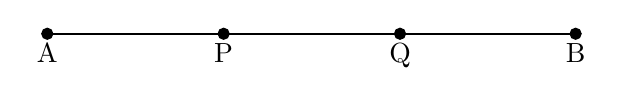
\begin{tikzpicture}
\draw[thick] 
    (-5.37, 4.92) --  % A
    (-3.13, 4.92) --  % P
    (-0.89, 4.92) --  % Q
    (1.34, 4.92) -- cycle;  % B
\node at (-5.37, 4.92) [below] {A};
\node at (-3.13, 4.92) [below] {P};
\node at (-0.89, 4.92) [below] {Q};
\node at (1.34, 4.92) [below] {B};
\filldraw 
    (-5.37, 4.92) circle (2pt)  % A
    (-3.13, 4.92) circle (2pt)  % P
    (-0.89, 4.92) circle (2pt)  % Q
    (1.34, 4.92) circle (2pt);  % B

\end{tikzpicture}
\end{figure}
\begin{center}
$\text{Figure } 2$
\end{center}
\begin{enumerate}
\item $2$\\
\item $4$\\
\item $-4$\\
\item $\frac{-5}{2}$\\
\end{enumerate}
%vectors
\item Find the value of $k$, if the point $P\brak{2,4}$ is equidistant from the points $A\brak{5,k}$ and $B\brak{k,7}$.\\
%vectors
\item Find the coordinates of a point $P$, which lies on the line segment joining the points $A\brak{-2,2}$ and $B\brak{2,-4}$ such that $AP = \frac{3}{7} AB$.\\
%vectors
\item The coordinates of the point $P$ dividing the line segment joining the points $A\brak{1,3}$ and $B\brak{4,6}$, in the ratio $2:1$ are:\\
\begin{enumerate}
\item $\brak{2,4}$\\
\item $\brak{3,5}$\\
\item $\brak{4,2}$\\
\item $\brak{5,3}$\\
\end{enumerate}
%vectors
\item If a point $A\brak{0,2}$ is equidistant from the points $B\brak{3,p}$ and $C\brak{p,5}$, then find the value of $p$.\\
%vectors
\item A point $P$ divides the line segment joining the points $A\brak{3,-5}$ and $B\brak{-4,8}$ such that $\dfrac{AP}{PB} = \dfrac{K}{1}$. If $P$ lies on the line $x + y = 0$, then find the value of $K$.\\
\item Find the ratio in which the line segment joining the points $\brak{1,-3}$ and $\brak{4,5}$ is divided by x-axis.\\
\item Find the ratio in which the y-axis divides the line segment joining the points \brak{5,-6}$ and \brak{-1,-4}$. Also find the coordinates of the point of intersection.\\
\item The area of a triangle whose vertices are $\brak{5,0}$, $\brak{8,0}$ and $\brak{8,4}$ $\brak{\text{in sq. units}}$ is\\
\begin{enumerate}
\item $20$\\
\item $12$\\
\item $6$\\
\item $16$\\
\end{enumerate}

\item If $A\brak{1,3}$, $B\brak{-1,2}$, $C\brak{2,5}$ and $D\brak{x,4}$ are the vertices of a parallelogram $ABCD$, then the value of $x$ is\\
\begin{enumerate}
\item $3$\\
\item $4$\\
\item $0$\\
\item $\frac{3}{2}$\\
\end{enumerate}

\item For what value of $k$, $\brak{ k > 0}$, s the area of the triangle with vertices $\brak{-2,5}$, \brak{k,-4}$, and \brak{2k+1,10}$ equal to $52$ sq. units?\\

\item If the vertices of a triangle are $\brak{1,-3}$, $\brak{4,p}$ and $\brak{-9,7}$ and its area is $15$ sq. units, find the value$\brak{\text{s}}$ of $p$.\\
\item Find the area of quadrilateral $ABCD$ whose vertices are $A\brak{-3,-1}$, $B\brak{-2,-4}$, $C\brak{4,-1}$ and $D\brak{3,4}$.\\

\item If the point $A\brak{x,y}$, $B\brak{3,6}$ and $C\brak{-3,4}$ are collinear, show that $x - 3y + 15 = 0$.\\
\end{enumerate}

\chapter{Circles}
\begin{enumerate}
\item From a point $Q$, $13 \text{ cm}$ away from the centre of a circle, the length of tangent $PQ$ to the circle is $12 \text{ cm}$. The radius of circle \brak{\text{in $cm$}}\\
\begin{enumerate}
\item $25$\\
\item $\sqrt{313}$\\
\item $5$\\
\item $1$\\
\end{enumerate}
%circles
\item In Figure $1$, $AP$, $AQ$ and $BC$ are tangents to the circle. If $AB = 5 \text{cm}$, $AC = 6 \text{ cm}$ and $BC = 4 \text{ cm}$, then the length of $AP$ \brak{\text{in $cm$}} is\\
\begin{figure} [h]
\centering
\begin{tikzpicture}[>=Stealth]

% Circle
\draw (0,0) circle (1cm);

% Points
\coordinate (A) at (0,3);
\coordinate (B) at (-0.7, 1);
\coordinate (C) at (0.7, 1);
\coordinate (P) at (-0.95, 0.3);
\coordinate (Q) at (0.95, 0.3);

% Tangents and Lines
\draw (A) -- (B) node[midway, left] {};
\draw (A) -- (C) node[midway, right] {};
\draw (B) -- (C) node[midway, below] {};
\draw (B) -- (P);
\draw (C) -- (Q);

% Arrows
\draw[->] (P) -- ($(B)!2cm!(P)$);
\draw[->] (Q) -- ($(C)!2cm!(Q)$);

% Perpendicular lines
\draw ($(P)!0.1cm!90:(B)$) -- ($(P)!0.1cm!-90:(B)$);
\draw ($(Q)!0.1cm!90:(C)$) -- ($(Q)!0.1cm!-90:(C)$);

% Labeling points
\node at (A) [above] {A};
\node at (B) [left] {B};
\node at (C) [right] {C};
\node at (P) [left] {P};
\node at (Q) [right] {Q};
\end{tikzpicture}
\end{figure}
\begin{center}
$\text{Figure } 1$
\end{center}
\begin{enumerate}
\item $7.5$\\
\item $15$\\
\item $10$\\
\item $9$\\
\end{enumerate}
%circles
\item The circumference of a circle is $22 \text{ cm}$. The area of its quadrant \brak{\text{in $cm^2$}}\\
\begin{enumerate}
\item $\frac{77}{2}$\\
\item $\frac{77}{4}$\\
\item $\frac{77}{8}$\\
\item $\frac{77}{16}$\\
\end{enumerate}
\item In Figure $3$, a right triangle $ABC$, circumscribe a circle of radius $r$. If $AB$ and $BC$ are of lengths $8 \text{ cm}$ and $6 \text{ cm}$ respectively, find the value of $r$.\\
\begin{figure}[ht]
\centering
\begin{tikzpicture}[scale=1]
    % Triangle ABC
    \coordinate[label=above:$A$] (A) at (0,8);
    \coordinate[label=below left:$B$] (B) at (0,0);
    \coordinate[label=below:$C$] (C) at (6,0);
    \draw (A) -- (B) -- (C) -- cycle;
    
    % Point (18/5, 16/5)
    \coordinate[label=above:$ $] (P) at (3.6,3.2);
    \fill (P) circle (0pt);
    
    % Line and length r
    \draw[thick] (2,2) -- (3.6,3.2);
    \node[label=below left:$O$,circle,fill,inner sep=1.5pt] (O) at (2,2) {};
    \node[label=above:$r$] at (2.8,2.6) {};
    \draw (O) circle (2cm);
    % Right angle at B
    \draw pic["$ $", draw=black, angle radius=0.4cm, angle eccentricity=1.5] {right angle = C--B--A};
\end{tikzpicture}
\end{figure}
\begin{center}
$\text{Figure } 3$
\end{center}
%Circles
\item Prove that the tangents drawn at the ends of a diameter of a circle are parallel.\\
%circles
\item In Figure $4$, $ABCD$ is a square of side $4 \text{ cm}$. A quadrant of a circle of radius $1 \text{ cm}$ is drawn at each vertex of the square and a circle of diameter $2 \text{ cm}$ is also drawn. Find the area of the shaded region. $\brak{\text{Use } \pi = 3.14}$\\
\begin{figure}[ht]
\centering
\begin{tikzpicture}
    % Draw the square
    \draw[thick] (0,0) rectangle (4,4);
    
    % Draw the circle
    \draw[thick,fill=white] (2,2) circle [radius=1];
    
    % Draw the quadrants
    \draw[thick,fill=white] (0,0) -- (1,0) arc [start angle=0, end angle=90, radius=1] -- cycle;
    \draw[thick,fill=white] (4,0) -- (3,0) arc [start angle=180, end angle=90, radius=1] -- cycle;
    \draw[thick,fill=white] (4,4) -- (3,4) arc [start angle=180, end angle=270, radius=1] -- cycle;
    \draw[thick,fill=white] (0,4) -- (1,4) arc [start angle=360, end angle=270, radius=1] -- cycle;
    
    % Add the hatching pattern with controlled density
    \path[pattern=north east lines, pattern color=black] (0,0) rectangle (4,4);
    
    % Exclude the circle and quadrants from the hatching by overlaying with white fill
    \draw[fill=white] (2,2) circle [radius=1];
    \draw[fill=white] (0,0) -- (1,0) arc [start angle=0, end angle=90, radius=1] -- cycle;
    \draw[fill=white] (4,0) -- (3,0) arc [start angle=180, end angle=90, radius=1] -- cycle;
    \draw[fill=white] (4,4) -- (3,4) arc [start angle=180, end angle=270, radius=1] -- cycle;
    \draw[fill=white] (0,4) -- (1,4) arc [start angle=360, end angle=270, radius=1] -- cycle;
    \node at (0,0) [below left] {A};
    \node at (4,0) [below right] {B};
    \node at (4,4) [above right] {C};
    \node at (0,4) [above left] {D};
\end{tikzpicture}
\end{figure}
\begin{center}
$\text{Figure } 4$
\end{center}
%Circles
\item From a rectangular sheet of paper $ABCD$ with $AB = 40 \text{ cm}$ and $AD = 28 \text{ cm}$, a semi-circular portion with $BC$ as diameter is cut off. Find the area of the remaining paper. $\brak{\text{Use } \pi = \frac{22}{7}}$\\
%Circles
\item In Figure $5$, a circle is inscribed in a triangle $PQR$ with $PQ = 10 \text{ cm}$, $QR = 8 \text{ cm}$ and $PR = 12 \text{ cm}$. Find the lengths of $QM$, $RN$ and $PL$.\\
\begin{figure}[ht]
\centering
\begin{tikzpicture}

% Define points
\coordinate (P) at (1.25,9.92);
\coordinate (Q) at (0,0);
\coordinate (R) at (8,0);
\coordinate (N) at (5.25,4);
\coordinate (L) at (0.33,2.9);
\coordinate (M) at (3,0);

% Draw triangle and lines
\draw[thick] (P) -- (Q) -- (R) -- cycle;
\draw[thick] (5.25,4) -- ++(0,-0.08) -- ++(0,0.3); % Perpendicular line at N
\draw[thick] (0.33,2.9) -- ++(-0.08,0) -- ++(0.2,0); % Horizontal line at (0.33,2.9)
\draw[thick] (3,0) -- ++(0,-0.08) -- ++(0,0.2); % Vertical line at M

% Draw incircle
\draw[thick] (3,2.64575) circle (2.64575cm);

% Labels
\node[above right] at (P) {P};
\node[below left] at (Q) {Q};
\node[below right] at (R) {R};
\node[below] at (M) {M};
\node[left] at (L) {L};
\node[above right] at (N) {N};

\end{tikzpicture}
\end{figure}
\begin{center}
$\text{Figure } 5$
\end{center}
%Circles
\item In Figure $6$, $O$ is the centre of the circle with $AC = 24 \text{ cm}$, $AB = 7 \text{ cm}$ and $\angle BOD = 90\degree$. Find the area of shaded region.$\brak{\text{Use } \pi = 3.14}$\\
%Circles
\item In Figure $7$, find the area of shaded region, if $ABCD$ is a square of side $14 \text{ cm}$ and $APD$ and $BPC$ are semicircles.\\
%circles
\item Prove that the length of tangents drawn from an external point to a circle are equal.\\
%circles
\item In Fig. $1$, the sides $AB$, $BC$ and $CA$ of a triangle $ABC$, touch a circle at $P$, $Q$ and $R$ respectively. If $PA = 4\text{ cm}$, $BP = 3\text{ cm}$ and $AC = 11\text{ cm}$, then the length of $BC$ \brak{\text{in $cm$}} is\\
\begin{enumerate}
\item $11$\\
\item $10$\\
\item $14$\\
\item $15$\\
\end{enumerate}
%circles
\item In Fig.$2$, a circle touches the side $DF$ of $\triangle EDF$ at $H$ and touches $ED$ and $EF$ produced at $K$ and $M$ respectively. If $EK = 9\text{ cm}$, then the perimeter of $\triangle EDF$ \brak{\text{in $cm$}} is\\
\begin{enumerate}
\item $18$\\
\item $13.5$\\
\item $12$\\
\item $9$\\
\end{enumerate}
%circles
\item If the area of a circle is equal to sum of the areas of two circles of diameters $10 \text{ cm}$ and $24 \text{ cm}$, then the diameter of the larger circle \brak{\text{in $cm$}} is\\
\begin{enumerate}
\item $34$\\
\item $26$\\
\item $17$\\
\item $14$\\
\end{enumerate}
%circles
\item The length of shadow of a tower on the plane ground is $\sqrt 3 \text{ m}$ times the height of the tower. The angle of elevation of sun is :\\
\begin{enumerate}
\item $45\degree$\\
\item $30\degree$\\
\item $60\degree$\\
\item $90\degree$\\
\end{enumerate}
%circles
\item If the coordinates of one end of a diameter of a circle are $\brak{2,3}$ and the coordinates of its centre are $\brak{-2,5}$, then the coordinates of the other end of the diameter are:\\
\begin{enumerate}
\item $\brak{-6,7}$\\
\item $\brak{6,-7}$\\
\item $\brak{6,7}$\\
\item $\brak{-6,-7}$\\
\end{enumerate}
%circles
\item Tangents $PA$ and $PB$ are drawn from an external point $P$ to two concentric circles with centre $O$ and radii $8 \text{ cm}$ and $5 \text{ cm}$ respectively, as shown in Fig.$3$. If $AP = 15\text{ cm}$, then find the length of $BP$.\\
%circles
\item In Fig.$4$, an isosceles triangle $ABC$, with $AB = AC$, circumscribe a circle. Prove that the point of contact $P$ bisects the base $BC$.\\
%circles
\item In Fig.$5$, the chord $AB$ of the larger of the two concentric circles, with centre $O$, touches the smaller circle at $C$. Prove that $AC = CB$.\\
%circles
\item In Fig.$6$, $OABC$ is a square of side $7 \text{ cm}$. If $OAPC$ is a quadrant of a circle with centre $O$, then find the area of the shaded region. $\brak{\text{Use } \pi = 3.14}$\\ 

%Circles
\item In Figure $3$, a right triangle $ABC$, circumscribe a circle of radius $r$. If $AB$ and $BC$ are of lengths $8 \text{ cm}$ and $6 \text{ cm}$ respectively, find the value of $r$.\\
\begin{figure}[ht]
\centering
\begin{tikzpicture}[scale=1]
    % Triangle ABC
    \coordinate[label=above:$A$] (A) at (0,8);
    \coordinate[label=below left:$B$] (B) at (0,0);
    \coordinate[label=below:$C$] (C) at (6,0);
    \draw (A) -- (B) -- (C) -- cycle;
    
    % Point (18/5, 16/5)
    \coordinate[label=above:$ $] (P) at (3.6,3.2);
    \fill (P) circle (0pt);
    
    % Line and length r
    \draw[thick] (2,2) -- (3.6,3.2);
    \node[label=below left:$O$,circle,fill,inner sep=1.5pt] (O) at (2,2) {};
    \node[label=above:$r$] at (2.8,2.6) {};
    \draw (O) circle (2cm);
    % Right angle at B
    \draw pic["$ $", draw=black, angle radius=0.4cm, angle eccentricity=1.5] {right angle = C--B--A};
\end{tikzpicture}
\end{figure}
\begin{center}
$\text{Figure } 3$
\end{center}
%Circles
\item Prove that the tangents drawn at the ends of a diameter of a circle are parallel.\\
%circles
\item In Figure $4$, $ABCD$ is a square of side $4 \text{ cm}$. A quadrant of a circle of radius $1 \text{ cm}$ is drawn at each vertex of the square and a circle of diameter $2 \text{ cm}$ is also drawn. Find the area of the shaded region. $\brak{\text{Use } \pi = 3.14}$\\
\begin{figure}[ht]
\centering
\begin{tikzpicture}
    % Draw the square
    \draw[thick] (0,0) rectangle (4,4);
    
    % Draw the circle
    \draw[thick,fill=white] (2,2) circle [radius=1];
    
    % Draw the quadrants
    \draw[thick,fill=white] (0,0) -- (1,0) arc [start angle=0, end angle=90, radius=1] -- cycle;
    \draw[thick,fill=white] (4,0) -- (3,0) arc [start angle=180, end angle=90, radius=1] -- cycle;
    \draw[thick,fill=white] (4,4) -- (3,4) arc [start angle=180, end angle=270, radius=1] -- cycle;
    \draw[thick,fill=white] (0,4) -- (1,4) arc [start angle=360, end angle=270, radius=1] -- cycle;
    
    % Add the hatching pattern with controlled density
    \path[pattern=north east lines, pattern color=black] (0,0) rectangle (4,4);
    
    % Exclude the circle and quadrants from the hatching by overlaying with white fill
    \draw[fill=white] (2,2) circle [radius=1];
    \draw[fill=white] (0,0) -- (1,0) arc [start angle=0, end angle=90, radius=1] -- cycle;
    \draw[fill=white] (4,0) -- (3,0) arc [start angle=180, end angle=90, radius=1] -- cycle;
    \draw[fill=white] (4,4) -- (3,4) arc [start angle=180, end angle=270, radius=1] -- cycle;
    \draw[fill=white] (0,4) -- (1,4) arc [start angle=360, end angle=270, radius=1] -- cycle;
\end{tikzpicture}
\end{figure}
\begin{center}
$\text{Figure } 4$
\end{center}
%Circles
\item From a rectangular sheet of paper $ABCD$ with $AB = 40 \text{ cm}$ and $AD = 28 \text{ cm}$, a semi-circular portion with $BC$ as diameter is cut off. Find the area of the remaining paper. $\brak{\text{Use } \pi = \frac{22}{7}}$\\
%Circles
\item In Figure $5$, a circle is inscribed in a triangle $PQR$ with $PQ = 10 \text{ cm}$, $QR = 8 \text{ cm}$ and $PR = 12 \text{ cm}$. Find the lengths of $QM$, $RN$ and $PL$.\\
%Circles
\item In Figure $6$, $O$ is the centre of the circle with $AC = 24 \text{ cm}$, $AB = 7 \text{ cm}$ and $\angle BOD = 90\degree$. Find the area of shaded region.$\brak{\text{Use } \pi = 3.14}$\\
%Circles
\item In Figure $7$, find the area of shaded region, if $ABCD$ is a square of side $14 \text{ cm}$ and $APD$ and $BPC$ are semicircles.\\
%circles
\item Prove that the length of tangents drawn from an external point to a circle are equal.\\
%circles
\item In Fig. $1$, the sides $AB$, $BC$ and $CA$ of a triangle $ABC$, touch a circle at $P$, $Q$ and $R$ respectively. If $PA = 4\text{ cm}$, $BP = 3\text{ cm}$ and $AC = 11\text{ cm}$, then the length of $BC$ \brak{\text{in $cm$}} is\\
\begin{enumerate}
\item $11$\\
\item $10$\\
\item $14$\\
\item $15$\\
\end{enumerate}
%circles
\item In Fig.$2$, a circle touches the side $DF$ of $\triangle EDF$ at $H$ and touches $ED$ and $EF$ produced at $K$ and $M$ respectively. If $EK = 9\text{ cm}$, then the perimeter of $\triangle EDF$ \brak{\text{in $cm$}} is\\
\begin{enumerate}
\item $18$\\
\item $13.5$\\
\item $12$\\
\item $9$\\
\end{enumerate}
%circles
\item If the area of a circle is equal to sum of the areas of two circles of diameters $10 \text{ cm}$ and $24 \text{ cm}$, then the diameter of the larger circle \brak{\text{in $cm$}} is\\
\begin{enumerate}
\item $34$\\
\item $26$\\
\item $17$\\
\item $14$\\
\end{enumerate}
%circles
\item The length of shadow of a tower on the plane ground is $\sqrt 3 \text{ m}$ times the height of the tower. The angle of elevation of sun is :\\
\begin{enumerate}
\item $45\degree$\\
\item $30\degree$\\
\item $60\degree$\\
\item $90\degree$\\
\end{enumerate}
%circles
\item If the coordinates of one end of a diameter of a circle are $\brak{2,3}$ and the coordinates of its centre are $\brak{-2,5}$, then the coordinates of the other end of the diameter are:\\
\begin{enumerate}
\item $\brak{-6,7}$\\
\item $\brak{6,-7}$\\
\item $\brak{6,7}$\\
\item $\brak{-6,-7}$\\
\end{enumerate}
%circles
\item Tangents $PA$ and $PB$ are drawn from an external point $P$ to two concentric circles with centre $O$ and radii $8 \text{ cm}$ and $5 \text{ cm}$ respectively, as shown in Fig.$3$. If $AP = 15\text{ cm}$, then find the length of $BP$.\\
%circles
\item In Fig.$4$, an isosceles triangle $ABC$, with $AB = AC$, circumscribe a circle. Prove that the point of contact $P$ bisects the base $BC$.\\
%circles
\item In Fig.$5$, the chord $AB$ of the larger of the two concentric circles, with centre $O$, touches the smaller circle at $C$. Prove that $AC = CB$.\\
%circles
\item In Fig.$6$, $OABC$ is a square of side $7 \text{ cm}$. If $OAPC$ is a quadrant of a circle with centre $O$, then find the area of the shaded region. $\brak{\text{Use } \pi = 3.14}$\\ 
%circles
\item Prove that the parallelogram circumscribing a circle is rhombus.\\
%circles
\item Prove that opposite sides of a quadrilateral circumscribing a circle subtend supplementary angles at the centre of the circle.\\
%circles
\item In Fig.$7$, $PQ$ and $AB$ are respectively the arcs of two concentric circles of radii $7\text{ cm}$ and $3.5\text{ cm}$ and centre $O$. If $\angle POQ = 30\degree$, then find the area of the shaded region. $\brak{\text{Use } \pi = \frac{22}{7}}$\\
\item $AB + CD = AD + BC$\\
Prove that the tangent at any point of a circle is perpendicular to the radius through the point of contact.\\

\item A quadrilateral $ABCD$ is drawn to circumscribe a circle. Prove that\\
$AB + CD = AD + BC$\\
\item In Figure $1$, $PQ$ and $PR$ are tangents to a circle with centre $A$. If $\angle QPA = 27\degree$, then $\angle QAR$ equals\\
\begin{enumerate}
\item $63\degree$\\
\item $153\degree$\\
\item $126\degree$\\
\item $117\degree$\\
\end{enumerate}
\item In Figure $2$, $AB$ and $AC$ are tangents to a circle with centre $O$ and radius $8\text{ cm}$. If $OA = 17\text{ cm}$, then the length of $AC \brak{\text { in cm}}$  is\\
\begin{enumerate}
\item $\sqrt {353}$\\
\item $15$\\
\item $9$\\
\item $25$\\
\end{enumerate}
\item In Figure $3$, three sectors of a circle of radius $7\text{ cm}$, making angles of $60\degree$, $80\degree$, $40\degree$ at the centre are shaded. The area of the shaded region $\brak{in\text{ cm}^2}$ is $\brak{\text{Using } \pi = \frac{22}{7}}$\\
\begin{enumerate}
\item $77$\\
\item $154$\\
\item $44$\\
\item $22$\\
\end{enumerate}
\item The incircle of an isosceles triangle $ABC$, with $AB = AC$, touches the sides $AB$, $BC$ and $CA$ at $D$, $E$ and $F$ respectively. Prove that $E$ bisects $BC$.\\

\item Prove that in two concentric circles. the chord of the larger circle, which touches the smaller circle, is bisected at the point of contact.\\

\item In Figure $4$, the shape of the top of the table is that of a sector of a circle with centre $O$ and $\angle OAB = 90\degree$. If $AO = OB = 42\text{ cm}$, then find the perimeter of the top of the table.\\

\item Find the area of the shaded region in Figure $5$, if $ABCD$ is a square of side $28\text{ cm}$ and $APD$ and $BPC$ are semicircles.\\
\item Two tangents $TP$ and $TQ$ are drawn to a circle with centre $O$ from an external point $T$. Prove that $\angle TPQ = 2\angle OPQ$.\\

\item In Figure $6$, $XY$ and $X'Y'$ are two parallel tangents to a circle with centre $O$ and another tangent $AB$ with point of contact $C$ intersects $XY$ at $A$ and $X'Y'$ at $B$. Prove that $\angle AOB = 90\degree$\\
\item In Figure $7$, $ABCD$ is a square of side $7\text{ cm}$. $DBPA$ and $DQBC$ are quadrants of circles, each of radius $7\text{ cm}$. Find the area of the shaded region.$\brak{\text{Use } \pi = \frac{22}{7}}$\\
\item The length of the minute hand of a clock is $14\text{ cm}$. Find the area swept by the minute hand in $10$ minutes. $\brak{\text{Use } \pi = \frac{22}{7}}$\\
\item Prove that the tangent at any point of a circle is perpendicular to the radius through the point of contact.\\
\end{enumerate}

\chapter{Discrete}
\begin{enumerate}
\item If the $n^{th}$ term of an $A.P$ is $\brak{2n+1}$, then sum of its first three terms is\\
\begin{enumerate}
\item $6n + 3$\\
\item $15$\\
\item $12$\\
\item $21$\\
\end{enumerate}
%discrete
\item Find the common difference of an $A.P$ whose first term is $5$ and the sum of its first four terms is half the sum of the next four terms.\\
%discrete
\item The $17th$ term of an $AP$ is $5$ more than twice its $8th$ term. If the $11th$ term of the $AP$ is $43$, then find the $nth$ term.\\

\item Sum of the first $14$ terms of an $AP$ is $1505$ and its first term is $10$. find its $25th$ term.\\
\item The next terms of $A.P.$ $\sqrt {18}, \sqrt {50}, \sqrt {98}, \ldots$ is\\
\begin{enumerate}
\item $\sqrt {146}$\\
\item $\sqrt {128}$\\
\item $\sqrt {162}$\\
\item $\sqrt {200}$\\
\end{enumerate}
\item In an $A.P.$, the first term is $12$ and the common difference is $6$. If the last term of the $A.P.$ is $252$, find its middle term.\\
\item If $4$ times the fourth term of an $A.P.$ is equal to $18$ times its $18^{th}$ term, then find its $22^{th}$ term.\\
\item The sum of $4^{th}$ and $8^{th}$ term terms of an $A.P.$ is $24$ and the sum of its $6^{th}$ and $10^{th}$ terms is $44$. Find the sum of first ten terms of the $A.P.$\\
\end{enumerate}

\chapter{Algebra}
\begin{enumerate}
\item The roots of the quadratic equation  $2x^2 - x - 6 = 0$ are\\
\begin{enumerate}
\item $-2,\frac{3}{2}$\\
\item $2,-\frac{3}{2}$\\
\item $-2,-\frac{3}{2}$\\
\item $2,\frac{3}{2}$\\
\end{enumerate}
%algebra
\item Find the value of $p$ for which the roots of the equation $px\brak{x-2} + 6 = 0$, are equal.\\
%Algebra
\item Solve the following quadratic equation for $x$ :\\
\begin{align}
x^2 - 4 a x - b^2 + 4a^2 = 0\\
\end{align}
%algebra
\item If $1$ is a root of the equations $ay^2 + ay + 3 = 0$ and $y^2 + y + b = 0$, then $ab$ equals :\\
\begin{enumerate}
\item $3$\\
\item $-\frac{7}{2}$\\
\item $6$\\
\item $-3$\\
\end{enumerate}
%algebra
\item Find the value$\brak{\text{s}}$ of $k$ so that the quadratic equation $x^2 - 4kx + k = 0$ has equal roots.\\
%algebra
\item Solve for $x$: $4x^2 - 4ax + \brak{a^2 - b^2} = 0$\\
%algebra
\item Solve for $x$: $3x^2 - 2\sqrt 6 x + 2 = 0$\\
\item If the quadratic equation $mx^2 + 2x + m = 0$ has two equal roots, then the values of $m$ are :\\
\begin{enumerate}
\item $\pm 1$\\
\item $0,2$\\
\item $0,1$\\
\item $-1,0$\\
\end{enumerate}

\item Find the value of $k$ for which the roots of the quadratic equation $\brak{k - 4} x^2 + 2\brak{k-4} x + 2 =0$ are equal.\\
\item Solve for x:\\
$4\sqrt 3 x^2 + 5x - 2\sqrt 3 = 0$\\
\end{enumerate}

\chapter{Probability}
\begin{enumerate}
\item Cards bearing numbers $2, 3, 4, \ldots, 11$ are kept in a bag. A card is drawn at random from the bag. The probability of getting a card with a prime number is\\
\begin{enumerate}
\item $\frac{1}{2}$\\
\item $\frac{2}{5}$\\
\item $\frac{3}{10}$\\
\item $\frac{5}{9}$\\
\end{enumerate}
%Probability
\item A card is drawn at random from a well shuffled pack of $52$ cards. Find the probability of getting\\
\begin{enumerate}[label=\Roman*.]
\item a red king.\\
\item a queen or a jack.\\
\end{enumerate}
%Probability
\item All kings, queens and aces are removed from a pack of $52$ cards. The remaining cards are well shuffled and then a card is drawn from it. Find the probability that the drawn card is \\
\begin{enumerate}[label=\Roman*.]
\item a black face card.\\
\item a red card.\\
\end{enumerate}
%probability
\item Two dices are thrown together. The probability of getting the same number on both dices is :\\
\begin{enumerate}
\item $\frac{1}{2}$\\
\item $\frac{1}{3}$\\
\item $\frac{1}{6}$\\
\item $\frac{1}{12}$\\
\end{enumerate}
%probability
\item A number is selected at random from first $50$ natural numbers. Find the probability that it is a multiple of $3$ and $4$.\\
%probability
\item A box contains $100$ red cards, $200$ yellow cards and $50$ blue cards. If a card is drawn at random from the box, then find the probability that it will be \begin{enumerate}[label=\Roman*.]
\item a blue card
\item not a yellow card
\item neither a yellow nor a blue card.\\
\end{enumerate}
\item The probability of a non-leap year having $53$ Mondays is \\
\begin{enumerate}
\item $\frac{2}{7}$\\
\item $\frac{1}{7}$\\
\item $\frac{5}{7}$\\
\item $\frac{6}{7}$\\
\end{enumerate}
\item A child has a die whose six faces show the letters as given below :\\
The die is thrown once. Find the probability of getting\\
\begin{enumerate}[label=\Roman*.]
\item A\\
\item D\\
\end{enumerate}
\item Cards marked with numbers $1,3,5, \ldots, 101$ are placed in a bag and mixed thoroughly. A card is then drawn at random from the bag. Find the probability that the number on the drawn card is 
\begin{enumerate}[label=\Roman*.]
\item less than $19$.
\item a prime number less than $20$.\\
\end{enumerate}
\end{enumerate}

\chapter{Trigonometry}
\begin{enumerate}
\item A kite is flying at a height of $30 \text{ m}$ from the ground. The length of string from the kite to the ground is $60 \text{ m}$. Assuming that there is no slack in the string, the angle of elevation of the kite at the ground is\\
\begin{enumerate}
\item $45\degree$\\
\item $30\degree$\\
\item $60\degree$\\
\item $90\degree$\\
\end{enumerate}
%Trigonometry
\item The angles of depression of the top and bottom of a tower as seen from the top of a $60\sqrt 3 \text{ m}$ high cliff are $45\degree$ and $60\degree$ respectively. Find the height of the tower.\\
%Trigonometry
\item In a flight of $2800 \text{ km}$, an aircraft was slowed down due to bad weather. Its average speed is reduced by $100 \text{ km/h}$ and time is increased by $30$ minutes. Find the original duration of flight.\\
%Trigonometry
\item The angles of elevation and depression of the top and bottom of a light-house from the top of a $60 \text{ m}$ high building are $30\degree$ and $60\degree$ respectively. Find\\
\begin{enumerate}[label=\Roman*.]
\item the difference between the heights of the light-house and the building.\\
\item the distance between light-house and building.\\
\end{enumerate}
%trigonometry
\item The angles of depression of two ships from the top of a light house and on the same side of it are found to be $45\degree$ and $30\degree$. if the ships are $200 \text{ km}$ apart, find the height of the light house.\\
\item The angle of elevation of the top of a hill at the foot of a tower is $60\degree$ and the angle of depression from the top of the tower of the foot of the hill is $30\degree$. If the tower is $50\text{ m}$ high, find the height of the hill.\\
\item From a point on the ground, which is $15\text{ m}$ away from the foot of a vertical tower, the angle of elevation of the top of the tower, is found to be $60\degree$. The height of the tower in $\brak{\text{in metres}}$ is\\
\begin{enumerate}
\item $5\sqrt 3$\\
\item $15\sqrt 3$\\
\item $15$\\
\item $7.5$\\
\end{enumerate}
\item From the top of a tower $50\text{ m}$ high, the angle of depression of the top of a pole is $45\degree$ and from the foot of the pole, the angle of elevation of the top of the tower is $60\degree$. find the height of the pole if the pole and tower stand on the same plane.\\
\item The angle of depression from the top of a tower of a point $A$ on the ground is $30\degree$. On moving a distance of $20\text{ m}$ from the point $A$ towards the foot of the tower to a point $B$ the angle of elevation of the top of the tower from point $B$ is $60\degree$. Find the height of the tower and its distance from point $A$.
\end{enumerate}

\chapter{Number Systems}
\input{number_sys.tex}
\chapter{Construction}
\begin{enumerate}
\item Draw a triangle $ABC$ with $BC = 7 \text{ cm}$, $\angle B = 45 \degree$ and $\angle C = 60 \degree$. Then construct another triangle, whose sides are $\frac{3}{5}$ times the corresponding sides of $\triangle ABC$.\\
%construction
\item Construct a right triangle in which the sides , (other than the hypotenuse) are of length $6\text{ cm}$ and $8\text{ cm}$. Then construct another triangle, whose sides are $\frac{3}{5}$ times the corresponding sides of the given triangle.\\
\item Draw a right triangle in which the sides (other than the hypotenuse) are of lengths $6\text{ cm}$ and $8\text{ cm}$. then construct another triangle whose sides are $\frac{3}{5}$ times the corresponding sides of the given triangle.\\
\end{enumerate}

\chapter{Geometry}
\begin{enumerate}
\item A solid right circular cone is cut into two parts at the middle of its height by a plane parallel to its base. The ratio of the volume of the smaller cone to the whole cone is\\
\begin{enumerate}
\item $1 : 2$\\
\item $1 : 4$\\
\item $1 : 6$\\
\item $1 : 8$\\
\end{enumerate}

\item A solid sphere of radius $10.5 \text{ cm}$ is melted and recast into smaller solid cones, each of radius $3.5 \text{ cm}$ and height $3 \text{ cm}$. Find the number of cones so formed. $\brak{\text{Use } \pi = \frac{22}{7}}$\\

\item A hemispherical bowl of internal radius $9 \text{ cm}$ is full of water. Its contents are emptied in a cylindrical vessel of internal radius $6 \text{ cm}$. Find the height of water in the cylindrical vessel.\\


\item A hemispherical tank, full of water, is emptied by a pipe at the rate of $\frac{22}{7}$ litres per sec. How much time will it take to empty half the tank if the diameter of the base of the tank is $3 \text{ m}$?\\

\item A drinking glass in the shape of the frustum of a cone of height $14 \text{ cm}$. The diameters of the two circular ends are $4 \text{ cm}$ and $2 \text{ cm}$. Find the capacity of the glass.  $\brak{\text{Use } \pi = 3.14}$\\

\item  A military tent of height $8.25 \text{ m}$ is in the form of a right circular cylinder of base diameter $30 \text{ m}$ and height $5.5 \text{ m}$ surmounted by a right circular cone of same base radius. Find the length of the canvas use in making tent, if the breadth of the canvas is $1.5 \text{ m}$.\\

\item If the radius of the base of a right circular cylinder is halved, keeping the height the same, then the ratio of the volume of the cylinder thus obtained to the volume of original cylinder is :\\
\begin{enumerate}
\item $1 : 2$\\
\item $1 : 4$\\
\item $2 : 1$\\
\item $4 : 1$\\
\end{enumerate}

\item The volume of a hemisphere is $2425\dfrac{1}{2}$ $\text{ cm}^3$. Find the curved surface area.  $\brak{\text{Use } \pi = 3.14}$\\

\item From a solid cylinder of height $7\text{ cm}$ and base diameter $12\text{ cm}$, a conical cavity of same height and same base diameter is hollowed out. Find the total surface area of the remaining solid. $\brak{\text{Use } \pi = \frac{22}{7}}$\\

\item A cylindrical bucket, $32 \text{ cm}$ high and with radius of base is $18 \text{ cm}$, is filled with sand. This bucket is emptied on the ground and a conical heap of sand is formed. If the height of the conical heap is $24 \text{ cm}$, then find the radius sand slant height of the heap.\\


\item A solid is in the shape of a cone surmounted on a hemisphere, the radius of each of them being $3.5\text{ cm}$ and the total height of solid is $9.5\text{ cm}$. Find the volume of the solid. $\brak{\text{Use } \pi = \frac{22}{7}}$\\

\item A bucket is in the form of a frustum of a cone and it can hold $28.499$ litres of water. If the radii of its circular ends are $28\text{ cm}$ and $21\text{ cm}$, find the height of the bucket. $\brak{\text{Use } \pi = \frac{22}{7}}$\\


\item The radii of a circular ends of a bucket of height $40\text{ cm}$ are $24\text{ cm}$ and $15\text{ cm}$. The slant height $\brak{\text{in cm}}$ of the bucket is\\
\begin{enumerate}
\item $51$\\
\item $49$\\
\item $43$\\
\item $41$\\
\end{enumerate}

\item A solid is in the shape of a cone mounted on a hemisphere of same base radius. If the curved surface area of the hemispherical part and the conical part are equal, then find the ratio of the radius and the height of the conical part.\\

\item A sphere of diameter $6\text{ cm}$ is dropped into a cylindrical vessel, partly filled with water, whose diameter is $12\text{ cm}$. If the sphere is completely submerged in water, by how much will the surface of water be raised in cylindrical vessel ?\\
\item A toy is in the shape of a cone mounted on a hemisphere of same base radius. If the volume of the toy is $231\text{ cm}^3$ and its diameter is $7\text{ cm}$, then find the height of the toy.  $\brak{\text{Use } \pi = \frac{22}{7}}$\\

\item The radii of internal and external surfaces of a hollow spherical shell are $3\text{ cm}$ and $5\text{ cm}$ respectively. It is melted and recast into a solid cylinder of diameter $14\text{ cm}$. Find the height of the cylinder.\\

\item A drinking glass is in the shape of a frustum of a cone of height $14\text{ cm}$. The diameters of its two circular ends are $16\text{ cm}$ and $12\text{ cm}$. Find the capacity of the glass. $\brak{\text{Use } \pi = \frac{22}{7}}$\\

\end{enumerate}


\section{2016}
\subsection{12}
\input{2016/Trigonometry.tex}
\section{2015}
\subsection{10}
\input{2015/trigo.tex}



%\chapter{Proofs}
%   \section{}
%\input{apps/defs.tex}

%  \section{}
%\input{apps/parab.tex}
%  \section{}
%\input{apps/nonparab.tex}
%		\section{}
%\input{apps/params.tex}
\latexprintindex

\end{document}

 
\section{Examples}
\subsection{Loney}
\input{examples/loney.tex}
\subsection{Miscellaneous}
\input{examples/misc.tex}
%
%%\section*{Disclosure Statement}
%%The authors report there are no competing interests to declare.
%%
%%
%%
%%  
%%%All the results related to conics are summarized in 
%%%Table \ref{table:conics}.  
%%%\begin{table*}[!t]
%%%\centering
%%%\input{conics.tex}
%%%%\input{./figs/conics.tex}
%%%\caption{$\vec{x}^{\top}\vec{V}\vec{x}+2\vec{u}^{\top}\vec{x}+f = 0$  can be expressed in the above standard form for various conics. $\vec{c}$ represents the centre/vertex of the conic. $\vec{q}$ is/are the point(s) of contact for the tangent(s). }
%%%\label{table:conics}
%%%\end{table*}
%%%\begin{verbatim}
%%\bibliographystyle{tfs}
%%%\bibliography{interacttfssample}
%%\bibliography{school}
%%\end{verbatim}
%% included where the list of references is to appear, where \texttt{tfs.bst} is the name of the \textsc{Bib}\TeX\ bibliography style file for Taylor \& Francis' Reference Style S and \texttt{interacttfssample.bib} is the bibliographic database included with the \textsf{Interact}-TFS \LaTeX\ bundle (to be replaced with the name of your own .bib file). \LaTeX/\textsc{Bib}\TeX\ will extract from your .bib file only those references that are cited in your .tex file and list them in the References section.
%
%% Please include a copy of your .bib file and/or the final generated .bbl file among your source files if your .tex file does not contain a reference list in a \texttt{thebibliography} environment.
%

  % \section{Appendices}
  % \appendix

\appendices
